\documentclass[titlepage]{article}

\usepackage{url}
\usepackage{tikz}
\usepackage{caption}

\title{Computer Workshop\\Assignment 2: Introduction to Git}
\author{Dr. MalekiMajd}
\date{Due: 22 Aban, 1402}

\newcommand{\code}{\texttt}

\begin{document}
\maketitle

\section*{Assignment Notes:}
\begin{enumerate}
    \item Some questions may include material not yet covered in class. These questions are meant to help you develop your research skills.
    \item Cheating or copying homework is strictly forbidden. If caught, both students involved will receive a score of 0 on this assignment.
    \item If you have any questions, feel free to ask in the course's Telegram group to benefit your fellow classmates.
    \item It's recommended to visit Git's official documentation for additional information on its commands.
\end{enumerate}

\pagebreak

\section{Basic Git Commands}
In this section, we'll delve into various Git commands and their optional arguments.

\subsection{\code{git add}}
\begin{enumerate}
    \item Let's take a closer look at the following commands:
    \begin{enumerate}
        \item \code{git add -u}
        \item \code{git add .}
        \item \code{git add -A}
    \end{enumerate}
    Explain each of these commands in detail.
    \item Why might the command \code{git add .} lead to a cluttered project directory structure?
\end{enumerate}

\subsection{\code{.gitignore}}
In this section, we'll explore the purpose of the \code{.gitignore} file.

\begin{enumerate}
    \item Describe the role of the \code{.gitignore} file in the root folder of your project.
    \item Explain when and why the \code{.gitignore} file can be valuable.
    \item What entries should you include in the \code{.gitignore} file to prevent tracking of all \code{.exe} files?
\end{enumerate}

\subsection{Other Git Commands}
\begin{enumerate}
    \item Explain the process of untracking a file that was previously tracked in Git.
\end{enumerate}

\section{Best Practices}
Read about good practices in Git at the following webpage and write down at least 5 good practices: \\ \url{https://gist.github.com/luismts/495d982e8c5b1a0ced4a57cf3d93cf60}

\pagebreak

\section{Project Structure}
In this section, you'll encounter two figures representing the structure of a project, with each node denoting a commit.

For each figure, provide all the necessary commands to create such a project. Remember to use the \code{git commit -am} command and make commits in the order of the nodes.

\begin{figure}[ht]
    \centering
    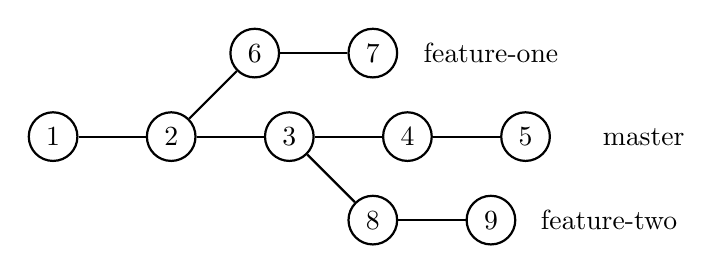
\begin{tikzpicture}[node distance={15mm}, thick, main/.style = {draw, circle}] 
        \node[main] (1) {1};
        \node[main] (2) [right of=1] {2};
        \node[main] (3) [right of=2] {3};
        \node[main] (4) [right of=3] {4};
        \node[main] (5) [right of=4] {5};
        \node[below left] (master) [right of=5] {master};
        \node[main] (6) [above right of=2] {6};
        \node[main] (7) [right of=6] {7};
        \node[below left] (feature-one) [right of=7] {feature-one};
        \node[main] (8) [below right of=3] {8};
        \node[main] (9) [right of=8] {9};
        \node[below left] (feature-two) [right of=9] {feature-two};
        
        \draw (1) -- (2);
        \draw (2) -- (3);
        \draw (3) -- (4);
        \draw (4) -- (5);
        
        \draw (2) -- (6);
        \draw (6) -- (7);
        
        \draw (3) -- (8);
        \draw (8) -- (9);
    \end{tikzpicture}
    \caption{Project 1}
    \label{fig:project1}
\end{figure}

\begin{figure}[ht]
    \centering
    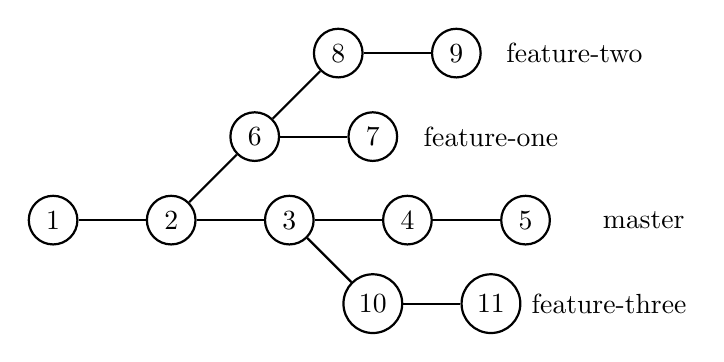
\begin{tikzpicture}[node distance={15mm}, thick, main/.style = {draw, circle}] 
        \node[main] (1) {1};
        \node[main] (2) [right of=1] {2};
        \node[main] (3) [right of=2] {3};
        \node[main] (4) [right of=3] {4};
        \node[main] (5) [right of=4] {5};
        \node[below left] (master) [right of=5] {master};
        \node[main] (6) [above right of=2] {6};
        \node[main] (7) [right of=6] {7};
        \node[below left] (feature-one) [right of=7] {feature-one};
        \node[main] (8) [above right of=6] {8};
        \node[main] (9) [right of=8] {9};
        \node[below left] (feature-two) [right of=9] {feature-two};
        \node[main] (10) [below right of=3] {10};
        \node[main] (11) [right of=10] {11};
        \node[below left] (feature-three) [right of=11] {feature-three};
        
        \draw (1) -- (2);
        \draw (2) -- (3);
        \draw (3) -- (4);
        \draw (4) -- (5);
        
        \draw (2) -- (6);
        \draw (6) -- (7);
        
        \draw (6) -- (8);
        \draw (8) -- (9);

        \draw (3) -- (10);
        \draw (10) -- (11);
    \end{tikzpicture}
    \caption{Project 2}
    \label{fig:project2}
\end{figure}

\end{document}

